\listfiles
\documentclass{article}

\usepackage[pdftex]{graphicx}
\usepackage{amsmath}
\usepackage{amssymb}

\usepackage[a4paper,margin=1in]{geometry}

\newcommand{\half}{\frac{1}{2}}
\newcommand{\D}{\Delta}

\title{The rainbow}
\date{}

\begin{document}
\maketitle

\section{The maximal diameter of a spherical water droplet}

We use spherical coordinates for this section, with the symbols $r$ for distance, $\theta$ for polar angle and $\phi$ for azimuthal angle. Since $r$ does not vary across our calculations, we set it to be $r = D/2$.

\subsection{Air resistant force}

The upward component of the force on a small section of area $dS$ is $f dS \sin \theta$. Hence the total upward force is

\begin{align*}
F_f &= \iint f dS \sin \theta \\
&= \iint f r^2 \sin\theta d\theta d\phi \sin\theta \\
&= r^2 f \int_0^\pi \sin^2 \theta d\theta \int_0^{2\pi} d\phi \\
&= r^2 f \frac{\pi}{2} 2\pi \\
&= \pi^2 r^2 f
\end{align*}

For constant speed this must balance the gravitational force

\begin{align*}
F_g &= \rho (\frac{4}{3} \pi r^3) g
\end{align*}

Hence

\begin{align*}
\pi^2 r^2 f &= \rho (\frac{4}{3} \pi r^3) g \\
\pi f &= \rho (\frac{4}{3} r) g \\
f &= \frac{4 \rho r g}{3\pi} \\
&= \frac{2 \rho D g}{3\pi}
\end{align*}

\subsection{Horizontal component of air resistant force}

The horizontal component of the air resistant force is

\begin{align*}
F_a &= \iint f dS \cos\theta \sin\phi \\
&= \iint f r^2 \sin\theta d\theta d\phi \cos\theta \sin\phi \\
&= r^2 f \int^{\frac{\pi}{2}}_\pi \sin\theta \cos\theta d\theta \int_0^\pi \sin\phi d\phi \\
&= r^2 f \\
&= \frac{D^2}{4} \frac{2 \rho D g}{3\pi} \\
&= \frac{\rho D^3 g}{6 \pi}
\end{align*}

\subsection{Surface tension}

The area of contact has a length $L = \pi D / 2$; hence $F_t = \sigma L$ 

\begin{align*}
F_t &= \frac{\sigma \pi D}{2}
\end{align*}

\subsection{Spherical water droplet}

\begin{align*}
F_t &= 100 F_a \\
\frac{\sigma \pi D}{2} &= 100 \frac{\rho D^3 g}{6 \pi} \\
\sigma \pi &= 100 \frac{\rho D^2 g}{3 \pi} \\
D &= \pi \sqrt{\frac{3 \sigma}{100 \rho g}} \\
&= 0.00277 \mathrm{\ m}
\end{align*}

The maximum diameter is 0.00277 m.

\section{Refraction and reflection of light rays in a spherical water droplet}

\subsection{Angle of reflected wave}

Let $\beta$ be the refracted angle; then

\begin{align*}
\sin\alpha &= n\sin\beta \\
\beta &= \sin^{-1}(\frac{1}{n} \sin\alpha)
\end{align*}

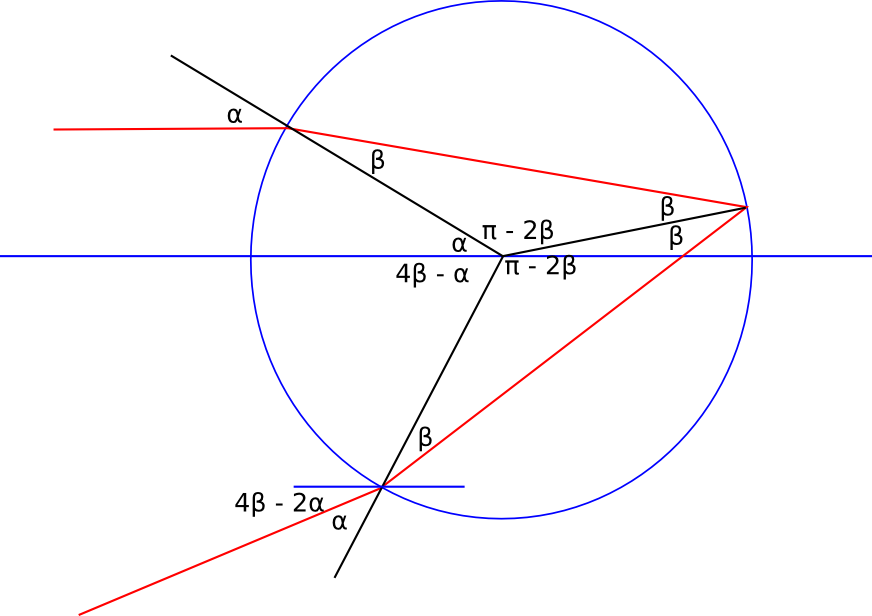
\includegraphics[width=\textwidth]{drawing.png}

\begin{align*}
\theta &= 4\beta - 2\alpha \\
&= 4 \sin^{-1}(\frac{1}{n} \sin\alpha) - 2\alpha
\end{align*}

[plot 4 * asin(0.74951 * sin(x)) - 2*x]

\subsection{Optical power distribution}

Let $x$ and $y$ be the coordinates of the incident beam, as seen when staring into the beam. Then

\begin{align*}
\D P &= I_0 \D x \D y
\end{align*}

a fraction $T_1 T_2 R$ of the beam is transmitted to the outgoing wave; hence we must relate $\D x$ and $\D y$ to $\D \theta$ and $\D \phi$. Now

\begin{align*}
\theta &= 4 \sin^{-1}(\frac{1}{n} \sin\alpha) - 2\alpha \\
\D\theta &= \left(\frac{4\cos\alpha}{n\sqrt{1 - (\frac{1}{n} \sin\alpha)^2}} - 2\right)\D\alpha
\end{align*}

and

\begin{align*}
r \sin\alpha &= y \\
r \cos\alpha \D\alpha &= \D y \\
\D\alpha &= \frac{\D y}{r \cos\alpha}
\end{align*}

so

\begin{align*}
\D\theta &= \left(\frac{4}{rn\sqrt{1 - (\frac{1}{n}\sin\alpha)^2}} - \frac{2}{r\cos\alpha}\right) \D y
\end{align*}

also, if we displace the beam a bit to the left or right (ie add $\D x$), $\alpha$ does not change to first order because the tangent to the circle of constant $\alpha$ is parallel to the direction of $\D x$ when $x$ is 0, as is the case here.

\begin{align*}
\D x &= \frac{r\sin\theta\sin\alpha}{\sin(4\beta - \alpha)} \D\phi
\end{align*}

Hence

\begin{align*}
\D P = I_0 \frac{\frac{r\sin\theta\sin\alpha}{\sin(4\beta - \alpha)} \D\phi}{\left(\frac{4}{rn\sqrt{1 - (\frac{1}{n}\sin\alpha)^2}} - \frac{2}{r\cos\alpha}\right)} \D\theta
\end{align*}

Therefore 

\begin{align*}
J &= I_0 \frac{\frac{\sin\theta\sin\alpha}{\sin(4\beta - \alpha)}}{\left(\frac{4}{n\sqrt{1 - (\frac{1}{n}\sin\alpha)^2}} - \frac{2}{\cos\alpha}\right)} T_1 T_2 R \\
&= I_0 \frac{\sin(4\sin^{-1}(\frac{1}{n} \sin\alpha)-2\alpha)\sin\alpha}{\sin(4\sin^{-1}(\frac{1}{n} \sin\alpha) - 2\alpha)\left(\frac{4}{n\sqrt{1 - (\frac{1}{n}\sin\alpha)^2}} - \frac{2}{\cos\alpha}\right)} T_1 T_2 R
\end{align*}

\subsection{$\lambda = 550 nm$}

[plot (sin(4*asin(0.74951 * sin(x))-2*x) * sin(x))/(sin(4 * asin(0.74951 * sin(x)) - 2*x) * (4/(1.3342 * sqrt(1 - (0.74951 * sin(x))**2)) - 2/(cos(x))))]

When we plot it, we see that it diverges at $\alpha = 1.04$; indeed, for this angle $\D \theta = 0$.

\subsection{Spectral Intensity}

\section{Basic characteristics of the rainbow}

\end{document}
